\section{Grundlagen}
%*Im Folgenden Kapitel werden die Grundlagen erklärt die Notwenig sind um die 
% Aufgabe zu verstehen. Es werden nur auf die Eigenschaften eingegangen die Nötig sind um die fortlaufende
%Arbeit zu verstehen. "Irgendwie so etwas in die richtung "
\subsection{Qubits} 
"`Der Anfang enthält also beides, Sein und
Nichts; ist die Einheit von Sein und Nichts,
– oder ist Nichtsein, das zugleich Sein, und
Sein, das zugleich Nichtsein ist."'
- Georg Wilhelm Friedrich Hegel

Die Repräsentation und Speicherung von Information ist ein zentraler Aspekt aller Computer, 
unabhängig von der verwendeten Technologie oder Architektur.
Heutzutage basieren klassische Computer in der Regel auf dem Binärsystem. 
In der klassischen Repräsentation ist das Bit die kleinste Informationseinheit, 
die eine von zwei mögliche Zustände annehmen kann: 0 oder 1. 
Ein Bit hat zu jedem Zeitpunkt einen klar definierten Zustand. 
Mehrmaliges Auslesen eines Bits führt zu keiner Zustandsänderung, 
sofern keine Operationen zwischen den Auslesungen durchgeführt werden.

Im Gegensatz dazu funktionieren Quantencomputer grundlegend anders. 
Sie stützen sich auf die Prinzipien der Quantenmechanik und 
verwenden anstelle von Bits sogenannte Quantenbits beziehungsweise Qubits zur Informationsrepräsentation. 
Ein einzelnes Qubit stellt die kleinstmögliche Informationseinheit dar, 
über die ein Quantencomputer verfügt. 
Um quantenmechanische Zustände von Qubits zu beschreiben, 
wird die Dirac-Notation als mathematische Schreibweise genutzt~\cite{dirac_1939}.

Ein Qubit kann den Zustand 0 oder den Zustand 1 annehmen:
\begin{center}
\(\ket{0}\) oder entsprechend \(\ket{1}\)
\end{center}

Des Weiteren kann ein Qubit auch beide der Basiszustände gleichzeitig einnehmen:
\begin{center}
\(\ket{\Psi} = \alpha\ket{0} + \beta\ket{1}\)
\end{center}
Dieses Phänomen ist eine der charakteristischen Eigenschaften von Qubits und wird als \textbf{Superposition} bezeichnet.
Dabei handelt es sich bei den Vorfaktoren \(\alpha\) und \(\beta\) um komplexe Zahlen, 
für die gilt:
\begin{center}
\(\lvert\alpha\rvert^2 + \lvert\beta\rvert^2 = 1\)
\end{center}
Es gibt also unendlich viele Zustände, die ein Qubit in einer Superposition der beiden Basiszustände annehmen kann.

In der klassischen Welt findet man nur schwer eine Analogie zur Superposition. 
Man kann sich dies jedoch in etwa an einer Münze vorstellen~\cite{Hoever2023Münze}:

Ein klassisches Bit kann dabei entweder auf der Kopf- oder auf der Zahl-Seite liegen.
Ein Qubit hingegen ist eine Münze, 
die auf der Kante um die eigene Achse rotiert.
Dabei geben die Vorfaktoren \(\alpha\) und \(\beta\) an,
wie die Münze zu der einen oder zu der anderen Seite tendiert.
Ohne die Münze zu beeinflussen, 
ist es nicht möglich, die Tendenz, 
also die Vorfaktoren, zu bestimmen.

Möchte man jedoch ein konkretes Ergebnis erhalten, 
muss man das Qubit lesen, 
beziehungsweise genauer gesagt messen.
Dabei wird die Superposition zerstört und das Qubit kollabiert in einen der beiden Basiszustände.

In Analogie zur Münze wird die Rotation der Münze gezielt gestoppt, sodass diese auf eine der beiden Seiten kippt.

Die Wahrscheinlichkeiten dafür werden durch die Vorfaktoren des Qubits bestimmt:
\begin{center}
\(\lvert\alpha\rvert^2\) für \(\ket{0}\), \(\lvert\beta\rvert^2\) für \(\ket{1}\)
\end{center}

Es ist also nicht möglich, 
den Zustand eines Qubit während einer Berechnung zu beobachten,
da ansonsten die Superposition zerstört wird und sich somit der Zustand des Qubits verändert.
Aus diesem Grund erfolgt die Messung in der Regel erst am Ende eines Quantenalgorithmus, um das endgültige Ergebnis zu ermitteln.

\subsection{Quantengatter}

\subsection{Qiskit}
\subsection{RSA}
%Funktionsweise
%Schwierigkeit Faktorisierung
%Laufzeit klassischer PC

\subsection{Quanten-Fourier-Transformation} \label{Quanten-Fourier-Transformation}
Die Quanten-Fourier-Transformation bildet einen wesentlichen Bestandteil des implementierten Quantenalgorithmus. 
Im folgenden Abschnitt wird die allgemeine Anwendung der Quanten-Fourier-Transformation erklärt.
Darüber hinaus wird die Implementierung des Quantenschaltkreises anhand der Formel der Quanten-Fourier-Transformation hergeleitet.

Im Prinzip handelt es sich bei der Quanten-Fourier-Transformation um eine Transformation,
die Qubits von der Standardbasis (\(\ket{0}\), \(\ket{1}\)),
in die entsprechende Fourierbasis (\(\ket{+}\), \(\ket{-}\)) überführt~\cite[215]{homeister2023quantum215}.
Bei dem Basiswechsel werden die Informationen des vorherigen Standardbasiszustands in die Phase des neuen Zustandes übertragen~\cite{Ruiz-Perez2017}.
Anschließend können in der Fourierbasis Rechnungen durchgeführt werden, 
die im Grunde durch Manipulationen der Phase realisiert werden.
Mit diesem Ansatz ist es möglich, arithmetische Operationen, wie beispielsweise 
die Addition, effizienter zu berechnen~\cite{draper2000addition,Ruiz-Perez2017}.

Unter Verwendung der inversen Quanten-Fourier-Transformation, 
die als Rücktransformation dient, ist es möglich, 
wieder zurück in die Standardbasis zu transformieren. 
Dies ermöglicht die Extraktion der Information aus der Phase in einen messbaren Zustand.

Die Quanten-Fourier-Transformation ist für ein \(N\) = \(2^n\) mit \(n\) Qubits
für die Basisvektoren \(\ket{x}, x = 0,...,N-1\) wie folgt definiert~\cite[216]{homeister2023quantum215}:
\[QFT_{N}\ket{x}_{n} = \frac{1}{\sqrt{N}}\sum_{y=0}^{N-1}  e^{\frac{2 \pi i x y}{N}}\ket{y}_{n}\]
Anhand dieser Definition kann der Quantenschaltkreis nicht direkt hergeleitet werden.
Stattdessen muss die Formel umgeformt werden.

Die folgende Herleitung stammt aus dem Lehrbuch \textit{Quantum Computation and Quantum Information}~\cite[218]{nielsen_chuang_2010}.
Der Übersicht halber werden Zwischenschritte hinzugefügt.

Indem \(y\) in der ersten Formel in die Binärschreibweise überführt wird, ergibt sich:
%Reihnfolge der Binärschreibweise einheitlich machen
% 
%\begin{align}
%    % -> & <-    &     ->&<-
%    122 &= 3     &   abc &= foo\\
%      x &= y     &
%      a &= 700   &
%\end{align}
%
%\begin{align}
% foo &= bar \\
%     &= baz \\
%     &= woop
%\end{align}
%
\[ y = \sum_{k=1}^{n}2^{n-k} y_{n-k+1}\]  
\begin{align}
  QFT_{N}\ket{x}_{n} &=
    \frac{1}{\sqrt{N}}
    \sum_{y_n=0}^{1} ...
    \sum_{y_1=0}^{1} e^{\frac{2 \pi i x \sum_{k=1}^{n}2^{n-k} y_{n-k+1}}{N}}
    \ket{y_n ... y_{2}y_{1}}
\end{align}
Mit \(N\) = \(2^n\) kann der Bruch im Exponenten gekürzt werden:
\[QFT_{N}\ket{x}_{n} = \frac{1}{\sqrt{N}}\sum_{y_n=0}^{1}...\sum_{y_1=0}^{1}  e^{\frac{2 \pi i x \sum_{k=1}^{n}2^{n-k} y_{n-k+1}}{2^n}}\ket{y_n ... y_{2}y_{1}}\]
\[QFT_{N}\ket{x}_{n} = \frac{1}{\sqrt{N}}\sum_{y_n=0}^{1}...\sum_{y_1=0}^{1}  e^{2 \pi i x \sum_{k=1}^{n}2^{-k} y_{n-k+1}}\ket{y_n ... y_{2}y_{1}}\]
Anschließend kann der Ausdruck \(2^{-k}\) zu \(\frac{1}{2^k}\) umgeformt werden: 
\[QFT_{N}\ket{x}_{n} = \frac{1}{\sqrt{N}}\sum_{y_n=0}^{1}...\sum_{y_1=0}^{1}  e^{\frac{2 \pi i x \sum_{k=1}^{n} y_{n-k+1}}{2^k}}\ket{y_n ... y_{2}y_{1}}\]
Die Summe im Exponenten der Basis \(e\) kann als Produkt umgeschrieben werden.
Anstatt dem Produktzeichen \(\prod\) wird das Tensorprodukt \(\Tensor\) verwendet, da es sich um Qubits handelt:
\[QFT_{N}\ket{x}_{n} = \frac{1}{\sqrt{N}}\sum_{y_n=0}^{1}...\sum_{y_1=0}^{1} \Tensor_{k=1}^n{ e^{\frac{2 \pi i x y_k}{2^k}}}\ket{y_{k}}\]
Der Ausdruck kann weiter vereinfacht werden indem das Tensorprodukt vorgezogen wird:
\[QFT_{N}\ket{x}_{n} = \frac{1}{\sqrt{N}}\Tensor_{k=1}^n [  \sum_{y_k=0}^{1}{ e^{\frac{2 \pi i x y_k}{2^k}}}\ket{y_{k}}]\]
\[QFT_{N}\ket{x}_{n} = \frac{1}{\sqrt{N}}\Tensor_{k=1}^n [  \ket{0} + { e^{\frac{2 \pi i x}{2^k}}}\ket{1}]\] 
Schreibt man das Tensorprodukt voll aus und notiert \(x\) in Binärschreibweise, erhält man:
\begin{align*}
\frac{1}{\sqrt{N}}\Bigg(
  \Big(\ket{0} + { e^{\frac{2 \pi i (2^{n-1}x_n+...+2^1x_2+2^0x_1)}{2^1}}}\ket{1}\Big)
  &\tensor
  \Big(\ket{0} + { e^{\frac{2 \pi i (2^{n-1}x_n+...+2^1x_2+2^0x_1)}{2^2}}}\ket{1}\Big) \\
  &\vdotswithin{\tensor} \\
  &\tensor
  \Big(\ket{0} + { e^{\frac{2 \pi i (2^{n-1}x_n+...+2^1x_2+2^0x_1)}{2^n}}}\ket{1}\Big)
  \Bigg)
\end{align*}
Die komplexe Exponentialfunktion ergibt für eine natürliche Zahl \(k\): \(e^{2\pi i k} = 1\).
Mit dieser Eigenschaft kann man beispielsweise die Phasenverschiebung des ersten Tensors vereinfachen:
\begin{align*} 
  e^{\frac{2 \pi i (2^{n-1}x_n+ \dotsb +2^1x_2+2^0x_1)}{2^1}}
  &\equiv
  e^{\frac{2 \pi i (2^{n-1}x_n)}{2^1}} \dotsb e^{\frac{2 \pi i (2^1x_2)}{2^1}} e^{\frac{2 \pi i (2^0x_1)}{2^1}} \\
  &\equiv 
  e^{{2 \pi i (2^{n-2}x_n)}} \dotsb e^{{2 \pi i (2^0x_2)}} e^{{2 \pi i (2^{-1}x_1)}}
\end{align*}
Dabei ergibt nur der Term \(e^{{2 \pi i (2^{-1}x_1)}} \neq 1 \)  
und verursacht somit eine relevante Phasenverschiebung.

Abschließend lässt sich das gesamte Tensorprodukt vereinfachen:
\begin{align*}
  QFT_{N}\ket{x}_{n} = 
  \frac{1}{\sqrt{N}}
  \Bigg(
    \Big(\ket{0} + { e^{\frac{2 \pi i (2^0x_1)}{2^1}}}\ket{1}\Big) 
    &\tensor
    \Big( \ket{0} + { e^{\frac{2 \pi i (2^1x_2+2^0x_1)}{2^2}}}\ket{1}\Big) \\
    &\vdotswithin{\tensor}\\
    &\tensor
    \Big( \ket{0} + { e^{\frac{2 \pi i (2^{n-1}x_n+ ... +2^1x_2+2^0x_1)}{2^n}}}\ket{1}\Big)
  \Bigg)
\end{align*}
Ein einzelner Tensor repräsentiert die Wirkung der Quantenschaltung auf ein einzelnes Qubit. 
Somit werden die Phasenverschiebungen erkennbar, 
die auf ein Qubit wirken. 
Außerdem verdeutlicht die Binärschreibweise, 
dass die angewendete Phasenverschiebung vom Zustand anderer Qubits abhängig ist.

Für die Implementierung der Quanten-Fourier-Transformation sind nur die Terme relevant, 
die eine Phasenverschiebung von ungleich 1 bewirken. 
Dies lässt sich mit der folgenden Formel beschreiben:
\[
QFT_{N}\ket{x}_{n} = \frac{1}{\sqrt{N}}
\Tensor_{k=1}^n \Big[  \ket{0} + { e^{\frac{2 \pi i \sum_{b=0}^{k-1}2^b x_{b+1} }{2^k}}}\ket{1}\Big]
\] 
Im Weiteren wird diese Formel verwendet, 
um einen Quantenschaltkreis für die Quanten-Fourier-Transformation mit drei Qubits zu implementieren:
\begin{align*}
QFT_{8}\ket{x}_{3} = 
\frac{1}{\sqrt{8}} 
  \Bigg[
    \Big(\ket{0} + { e^{\frac{2 \pi i (2^0x_1)}{2^1}}}\ket{1} \Big) 
    &\tensor
    \Big(\ket{0} + { e^{\frac{2 \pi i (2^1x_2+2^0x_1)}{2^2}}}\ket{1} \Big) \\
    &\tensor
    \Big(\ket{0} + { e^{\frac{2 \pi i (2^{2}x_3 +2^1x_2+2^0x_1)}{2^3}}}\ket{1} \Big) 
  \Bigg] 
\end{align*}
Man kann die durch den Eingangszustand eines einzelnen Qubits erzeugte Phasenverschiebung verdeutlichen, 
indem man die Addition im Exponenten zu einer Multiplikation der gleichen Basen umformt:
\begin{align*}
  QFT_{8}\ket{x}_{3} = 
  \frac{1}{\sqrt{8}} 
  \Bigg[
    \Big(\ket{0} + { e^{\frac{2 \pi i (2^0x_1)}{2^1}}}\ket{1}\Big) 
    &\tensor
    \Big(\ket{0} + { e^{\frac{2 \pi i (2^1x_2)}{2^2}} e^{\frac{2 \pi i (2^0x_1)}{2^2}} }\ket{1} \Big) \\ 
    &\tensor
    \Big(\ket{0} + { e^{\frac{2 \pi i (2^{2}x_3)}{2^3}} e^{\frac{2 \pi i (2^1x_2)}{2^3}} e^{\frac{2 \pi i (2^0x_1)}{2^3}}  }\ket{1} \Big)
  \Bigg] 
\end{align*}
Die wirkenden Phasenverschiebungen werden eindeutiger, 
indem man die Brüche kürzt:
\begin{align*}
  QFT_{8}\ket{x}_{3} = 
  \frac{1}{\sqrt{8}} 
  \Bigg[ 
    \Big( \ket{0} + e^{\pi i x_1}\ket{1} \Big) \tensor
    \Big(\ket{0} + { e^{\pi i x_2} e^{ \frac{ \pi i x_1}{2}} }\ket{1} \Big) \tensor
    \Big(\ket{0} + { e^{\pi i x_3} e^{\frac{\pi i x_2}{2}} e^{ \frac{ \pi i x_1}{4}} }\ket{1} \Big) 
  \Bigg] 
\end{align*}
In einer abschließenden Umformung lässt sich der Bruch \(\frac{1}{\sqrt8}\) aufteilen.
Dadurch erinnern die einzelnen Tensoren,
beziehungsweise Qubits an die Form die durch eine Hadamard-Transformation entsteht:
\begin{align*}
  QFT_{8}\ket{x}_{3} = 
   \frac{1}{\sqrt{2}}\Big( \ket{0} + e^{\pi i x_1}\ket{1} \Big) 
   &\tensor
  \frac{1}{\sqrt{2}}\Big( \ket{0} + { e^{\pi i x_2} e^{ \frac{ \pi i x_1}{2}} }\ket{1} \Big) \\ 
  &\tensor
  \frac{1}{\sqrt{2}}\Big( \ket{0} + { e^{\pi i x_3} e^{\frac{\pi i x_2}{2}} e^{ \frac{ \pi i x_1}{4}} }\ket{1} \Big)  
\end{align*}
Der Ausdruck \(e^{\pi i x_k}\) ist in jedem der einzelnen Qubits vorhanden.
Des Weiteren ist an dem \(x_k\) erkennbar, 
dass die angewendete Phasenverschiebung vom Eingangszustand des Qubits abhängt,
auf das die Verschiebung auch angewendet wird. 
Konkret bedeutet dies, 
dass auf jedes Qubit mit dem Zustand \(\ket{x_k} = \ket{1}\) eine Phasenverschiebung von \(e^{\pi i}\) wirkt.
Anhand des ersten Qubits, 
beziehungsweise des ersten Tensors, 
ergibt sich bei \(x_1 = 0\)
der Zustand \(\ket{0} + e^{\pi i 0} \ket{1} \equiv \ket{0} + \ket{1}\).
Bei \(x_1 = 1\) erhält man \(\ket{0} + e^{\pi i 1} \ket{1}\),
was \(\ket{0} - \ket{1}\) entspricht.
Aufgrund des Vorfaktors von \(\frac{1}{\sqrt{2}}\) entsprechen beide Fälle also der Hadamard-Transformation.
Da alle anderen Tensoren ebenfalls den Ausdruck \(e^{\pi i x_k}\) 
und den Vorfaktor \(\frac{1}{\sqrt{2}}\) beinhalten, 
wirkt auf jedes Qubit ein Hadamard-Gatter.

Die weiteren Tensoren des Tensorprodukts beinhalten zunehmend mehr Ausdrücke, 
die für unterschiedliche Phasenverschiebungen sorgen. 
Die Phasenverschiebung eines einzelnen Ausdrucks kann mit einem Phasengatter realisiert werden. 
Das Phasengatter entspricht der Rotation:
\[
  P(\lambda) = 
  \begin{pmatrix}
    1 & 0 \\
    0 & e^{i \lambda}
  \end{pmatrix}
\]

Beispielsweise wirkt auf das zweite Qubit ein Phasengatter mit \(P(\frac{\pi}{2} )\).
Diese Phasenverschiebung soll jedoch nur angewendet werden, 
wenn \(x_1 = 1\) ist.
Aus diesem Grund wird das Phasengatter durch den Eingangszustand des ersten Qubits gesteuert und 
mithilfe eines kontrollierten Phasengatters realisiert.
Das gleiche Prinzip gilt für alle weiteren Qubits.
Anschließend ergibt sich ein Quantenschaltkreis, 
wie er in Abbildung~\ref{fig:qft} dargestellt ist.

Wie aus Abbildung~\ref{fig:qft} ersichtlich, 
kehrt die Quanten-Fourier-Transformation die Reihenfolge der Qubits um~\cite[217]{homeister2023quantum215}.
Um die ursprüngliche Reihenfolge wiederherzustellen, 
werden am Ende der Quanten-Fourier-Transformation Swap-Operationen durchgeführt.
\begin{figure} [H]
\caption{3-Qubit QFT}
\label{fig:qft}
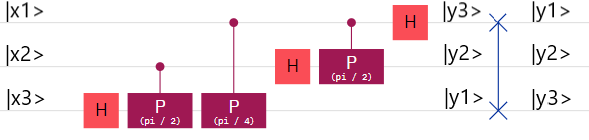
\includegraphics[width=\columnwidth]{qft.PNG}
\centering
\end{figure}

Anhand der Implementierung wird ersichtlich,
dass die Quanten-Fourier-Transformation unitär ist. 
Diese Eigenschaft ergibt sich aus der Tatsache, 
dass der zugehörige Quantenschaltkreis ausschließlich unter Verwendung von unitären Gattern realisierbar ist.

Wie bereits oben erwähnt, 
wird für die Rücktransformation aus der Fourierbasis in die Standardbasis die inverse Quanten-Fourier-Transformation angewendet.
Um einen Quantenschaltkreis aus unitären Gattern zu invertieren, 
werden die Inversen der verwendeten Gatter in umgekehrter Reihenfolge zur ursprünglichen Schaltung angewendet. 
Die Swap-Operationen stehen somit bei der inversen Quanten-Fourier-Transformation am Anfang.
In Abbildung~\ref{fig:iqft} ist beispielhaft die inverse Quanten-Fourier-Transformation für drei Qubits abgebildet.
\begin{figure} [H]
\caption{3-Qubit inverse QFT}
\label{fig:iqft}
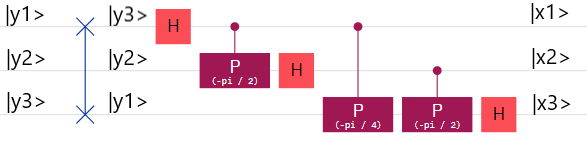
\includegraphics[width=\columnwidth]{iqft.PNG}
\centering
\end{figure}

\subsection{Quanten-Phase-Estimation} \label{Quanten-Phase-Estimation}

Im nachfolgenden Abschnitt wird die Anwendung und Funktionsweise des Quantum-Phase-Estimation Quantenalgorithmus erläutert. 
Die Quantum-Phase-Estimation ist ein Bestandteil einiger fortgeschrittener Quantenalgorithmen und eine integrale Komponente des spezifischen Quantenalgorithmus, 
der in dieser Arbeit implementiert wird. 
Genauer gesagt, 
basiert der implementierte Algorithmus auf den Prinzipien der Quantum-Phase-Estimation und verwendet dieselbe Methodik für einen spezialisierten Kontext.

Schwerpunktmäßig konzentriert sich die Erklärung primär auf das Verständnis der Funktionsweise der Quantum-Phase-Estimation und nimmt an, 
dass einige Voraussetzungen gegeben sind. 
Diese Voraussetzungen hängen vom spezifischen Kontext ab, 
in dem die Quantum-Phase-Estimation angewendet wird. 
Im weiteren Verlauf der Arbeit werden diese Voraussetzungen im Hinblick auf den Anwendungsfall des implementierten Quantenalgorithmus konkretisiert.

Eine der Voraussetzungen ist, 
dass ein Eigenvektor \(\ket{x}_n\) einer unitären Transformation \(U^{n\times n}\) bekannt ist.
Wendet man die Transformation \(U^{n\times n}\) auf \(\ket{x}_n\) an, 
so gilt~\cite[221]{nielsen_chuang_2010}: 
\[U^{n\times n}\ket{x}_n=\lambda_x\ket{x}_n\]
Dabei erhält man, abhängig vom gewählten Eigenvektor \(\ket{x}_n\), einen der Eigenwert \(\lambda_x\) von \(U^{n\times n}\).
Ein Eigenwert \(\lambda_x\) besitzt die Form eines Phasenfaktors: \(e^{2\pi i \varphi}\),
mit \(0 \leq \varphi < 1\).
Im Prinzip wird durch die unitäre Transformation also eine globale Phasenverschiebung auf den Eigenvektor angewendet.

Wie bereits im Kapitel zu den Grundlagen gezeigt wurde, 
ist es nicht möglich, eine globale Phase durch eine gewöhnliche Messung der Qubits zu bestimmen. 
Das liegt daran, dass eine globale Phase die Amplituden eines Qubits nicht verändert und 
somit die Wahrscheinlichkeiten der Messergebnisse unverändert bleiben. 
Stattdessen muss man die Qubits so manipulieren, 
dass die globale Phase doch Einfluss auf die Amplituden nimmt.

Der Quanten-Phase-Estimation Quantenalgorithmus ist in der Lage, 
den Eigenwert aus \(U^{n\times n}\ket{x}_n=\lambda_x\ket{x}_n\), 
also die Phasenverschiebungen repräsentiert durch \(\lambda_x = e^{2\pi i \varphi}\),
auf die Amplitude eines anderen Qubits zu verschieben.
Um \(\lambda_x\) auf ein anderes Qubit zu übertragen, 
wird der Effekt des \textbf{Phase-Kickback} genutzt.
Anschließend wird der Wert \(\varphi\) des Eigenwertes durch die inverse Quanten-Fourier-Transformation in einen messbaren Zustand überführt.

Der Phase-Kickback tritt auf, 
wenn eine unitäre Transformation \(U^{n\times n}\), die durch ein Qubit \(\ket{y}_1\) in Superposition kontrolliert wird,
auf einen Eigenvektor \(\ket{x}_n\) von \(U^{n\times n}\) anwendet wird.
Dabei wird der Eigenwert, genauer gesagt \(\lambda_x\), 
auf den \(\ket{1}\)-Anteil von \(\ket{y}_1\) übertragen.

Sei \( \ket{y}_1 = \alpha\ket{0} + \beta\ket{1} \) mit \( \alpha,\beta \neq 0 \), dann gilt:
\begin{align*}
  CU^{(n+1)\times (n+1)}(\ket{y}_1 \otimes \ket{x}_n) 
  &= CU^{(n+1)\times (n+1)}\big((\alpha\ket{0} + \beta\ket{1}) \otimes \ket{x}_n\big) \\
  &= CU^{(n+1)\times (n+1)}\big((\alpha\ket{0}\otimes\ket{x}_n) + (\beta\ket{1}\otimes \ket{x}_n)\big) \\
  &= \big((\alpha\ket{0}\otimes\ket{x}_n) + (\beta\ket{1}\otimes U^{(n)\times (n)}\ket{x}_n)\big) \\
  &= \big((\alpha\ket{0}\otimes\ket{x}_n) + (\beta\ket{1}\otimes \lambda_x\ket{x}_n)\big) \\
  &= (\alpha\ket{0} + \lambda_x\beta\ket{1}) \otimes \ket{x}_n
\end{align*}
In der Rechnung wird also die globale Phase \(\lambda_x\) von \(\ket{x}_n\) als relative Phase auf \(\ket{y}_1\) übertragen.

Es folgt ein Beispiel welches den Effekt verdeutlicht:
Beachtet werden zwei Qubits im Zustand \(\ket{+}_1 \tensor \ket{-}_1\) auf die ein kontrolliertes X-Gatter angewendet wird.
Dabei ist \(\ket{-}_1\) der Eigenvektor einer X-Transformation mit zugehörigen Eigenwert \(-1\), also: 
\[X^{1\times 1}\ket{-}_1=-\ket{-}_1\]
Auf das zweite Qubit \(\ket{-}_1\) wirkt ein \(CX^{2\times 2}\) Gatter welches durch das erste Qubit \(\ket{+}_1\) kontrolliert wird:
\[
  CX^{2\times 2}( \ket{+}_1\ \tensor \ket{-}_1) =
  \begin{pmatrix}
    1 & 0 & 0 & 0\\
    0 & 1 & 0 & 0\\
    0 & 0 & 0 & 1\\
    0 & 0 & 1 & 0
  \end{pmatrix}
  \cdot
  \frac{1}{{2}}
  \begin{pmatrix}
    1 \\
    -1 \\
    1 \\
    -1 
  \end{pmatrix}
  =
  \frac{1}{{2}}
  \begin{pmatrix}
    1 \\
    -1 \\
    -1 \\
    1 
  \end{pmatrix}
  \]
  \[
  =
  \frac{1}{{\sqrt{2}}}
  \begin{pmatrix}
    1 \\
    -1 
  \end{pmatrix}
  \tensor
  \frac{1}{{\sqrt{2}}}
  \begin{pmatrix}
    1 \\
    -1 
  \end{pmatrix}
  =
  \ket{-}_1 \tensor \ket{-}_1
  \]
Mit Hilfe des Phase-Kickback kann man also den Eigenwert einer unitären Transformation in die relative Phase eines Kontrollqubits verschieben.
Der Vorteil davon ist, 
dass diese Phasenverschiebung nur den Vorfaktor von \(\ket{1}\) des Kontrollqubits betrifft und keine globale Phase darstellt.

Der Aufbau eines Quanten-Phase-Estimation Quantenschaltung sieht beispielsweise wie folgt aus:
Beachtet wird die unitäre Transformation eines Phase-Gatter(P) mit einer variablen Phasenverschiebung von 
\[P(2 \pi \varphi ) = 
\begin{pmatrix}
  1 & 0\\
  0 & e^{2 i \pi \varphi}
\end{pmatrix}\]
Ein zugehöriger Eigenvektor dieser Transformation ist \(\ket{1}_1\), 
den: 
\[P(2 \pi \varphi)\ket{1}_1 = e^{2 i \pi \varphi} \ket{1}_1\]

Um den Effekt des Phase-Kickback nutzen zu können, 
muss sich das Kontrollqubit in einer Superposition befinden.
Dafür wird das Kontrollqubit im Zustand \(\ket{0}_1\) initialisiert und
anschließend mit einem Hadamard-Gatter(H) in die gleichmäßige Superposition \(\ket{+}_1\) versetzt.
\[\ket{0}_1 \tensor \ket{1}_1 
\underrightarrow{H^{\tensor 1}}
 \ket{+}_1 \tensor \ket{1}_1
=
\frac{1}{\sqrt{2}}
\begin{pmatrix}
  1 \\
  1
 \end{pmatrix}
 \tensor
 \begin{pmatrix}
  0 \\
  1 
 \end{pmatrix}
 =
 \frac{1}{\sqrt{2}}
 \begin{pmatrix}
  0 \\
  1 \\
  0 \\
  1
\end{pmatrix}
 \]
Über das kontrollierte Phase-Gatter wird der Eigenwert auf das Kontrollqubit verschoben und
befindet sich daher nicht mehr im Zustand \(\ket{+}_1\) :
\[
  \frac{1}{\sqrt{2}}
  \begin{pmatrix}
   0 \\
   1 \\
   0 \\
   1
  \end{pmatrix}
  \underrightarrow{CP^{2\times 2}(2 \pi \varphi)}
  \begin{pmatrix}
    1 & 0 & 0 & 0\\
    0 & 1 & 0 & 0\\
    0 & 0 & 1 & 0\\
    0 & 0 & 0 & e^{2 i \pi \varphi}
  \end{pmatrix}
  \cdot
  \frac{1}{\sqrt{2}}
  \begin{pmatrix}
   0 \\
   1 \\
   0 \\
   1
  \end{pmatrix}
  =
  \frac{1}{\sqrt{2}}
  \begin{pmatrix}
    0 \\
    1 \\
    0 \\
    e^{2 i \pi \varphi}
  \end{pmatrix}
  =
  \frac{1}{\sqrt{2}}
  \begin{pmatrix}
    1 \\
    e^{2 i \pi \varphi}
   \end{pmatrix}
   \tensor
   \begin{pmatrix}
    0 \\
    1 
   \end{pmatrix}
  \]
Anschließend wird auf die Kontrollqubits die inverse Quanten-Fourier-Transformation angewendet.
Die inverse Quanten-Fourier-Transformation sorgt dafür, 
dass der Eigenwert die Amplituden der Kontrollqubits beeinflusst.
Die Qubits mit dem Eigenvektor sind für den weiteren Ablauf der Quanten-Phasen-Estimation nicht mehr relevant 
und werden nicht weiter beachtet.
Im vorliegenden Beispiel entspricht die inverse Quanten-Fourier-Transformation einem Hadamard-Gatter, da lediglich ein Kontrollqubit vorhanden ist:
\[
\frac{1}{\sqrt{2}}
\begin{pmatrix}
  1 \\
  e^{2 i \pi \varphi}
 \end{pmatrix}
 \underrightarrow{H^{\tensor 1}}
 \frac{1}{\sqrt{2}}
 \begin{pmatrix}
  1 & 1\\
  1 & -1
 \end{pmatrix}
 \cdot
 \frac{1}{\sqrt{2}}
\begin{pmatrix}
  1 \\
  e^{2 i \pi \varphi}
 \end{pmatrix}
 =
 \frac{1}{2}
 \begin{pmatrix}
  1 + e^{2 i \pi \varphi}\\
  1 - e^{2 i \pi \varphi}
 \end{pmatrix}
\]
Das Ergebnis des Beispiels zeigt, dass der Eigenwert praktisch auf die Amplitude vom Kontrollqubit transformiert wird.

Verwendet man ein Phase-Gatter mit \(\varphi  = 0.075\), 
so sieht der Quantenschaltkreis wie in Abbildung~\ref{fig:qpe_1qubit} aus.
\begin{figure}[H]
  \caption{Einzelnes Kontroll-Qubit QPE}
  \label{fig:qpe_1qubit}
  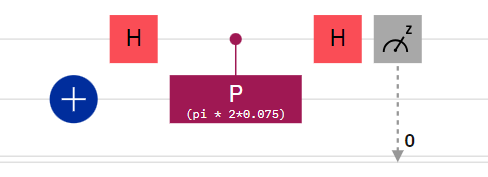
\includegraphics[ scale = 0.9]{qpe_1qubit.PNG}
  \centering
  \end{figure}
Mit dieser Phasenverschiebung sollte man bei einer Messung den Zustand \(\ket{0}\)
mit einer Wahrscheinlichkeit von ungefähr \(0.9455\) 
und den Zustand \(\ket{1}\) mit der Wahrscheinlichkeit \(0.0544\) erhalten.
Die Ergebnisse von 20.000 Messungen, dargestellt in Abbildung~\ref{fig:qpe_1qubit_Messung}, 
bestätigen die Größenordnung dieser Wahrscheinlichkeiten.
Jedoch entsprechen die Messungen aus Abbildung~\ref{fig:qpe_1qubit_Messung} nicht ganz den theoretisch ausgerechneten Wahrscheinlichkeiten.
Dies liegt an der probabilistischen Natur der Messung.
Bei einer zunehmenden Anzahl an Messungen würden die Ergebnisse gegen die theoretisch erwarteten Wahrscheinlichkeitswerte konvergieren.
Somit sind viele Durchläufe des Quantenalgorithmus erforderlich, 
um anhand der Messungen ein verlässliches Ergebnis zu erhalten.
\begin{figure}[H]
  \caption{Einzelnes Kontroll-Qubit QPE Messung}
  \label{fig:qpe_1qubit_Messung}
  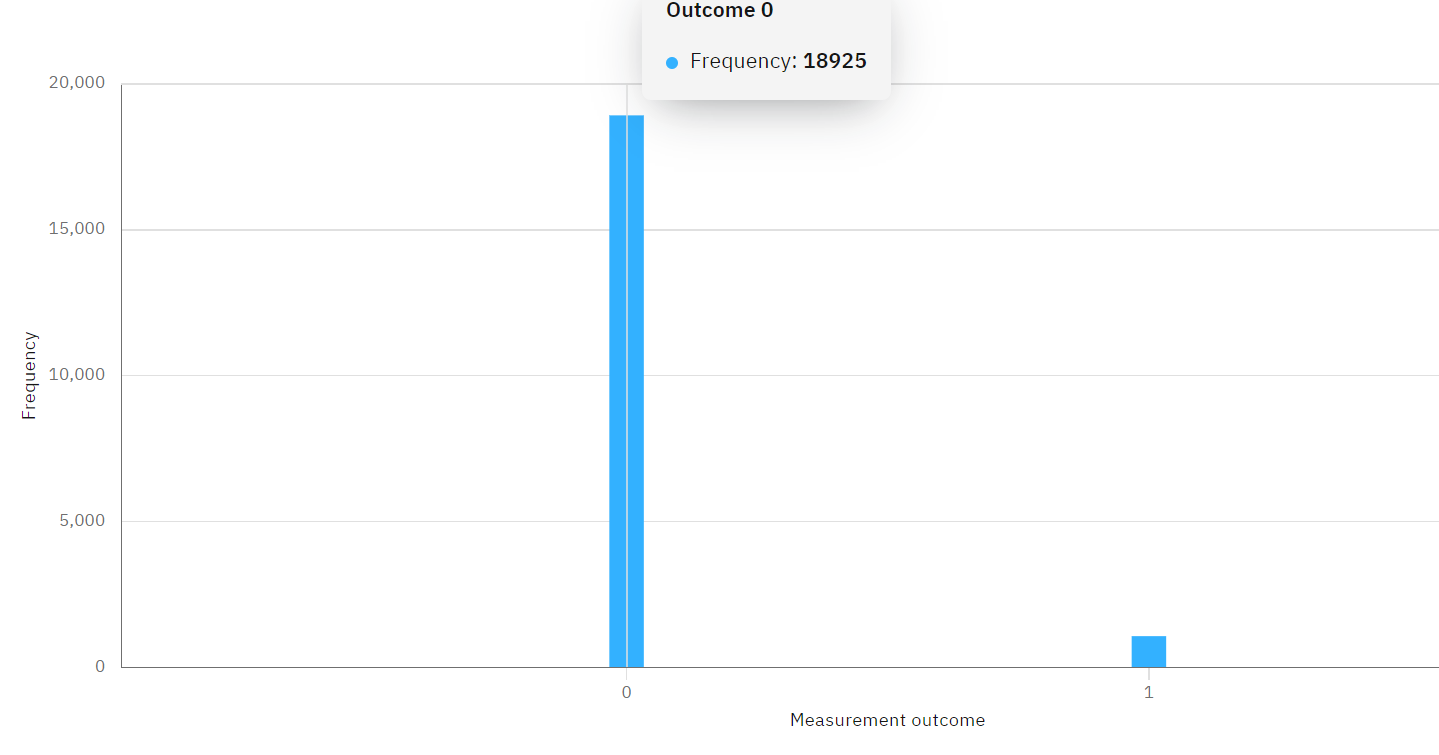
\includegraphics[width=\columnwidth]{qpe_1qubit_Messung.PNG}
  \centering
  \end{figure}
  

Die Präzision der Quanten-Phasenabschätzung lässt sich durch die Verwendung mehrerer Qubits erhöhen.
Diese zusätzlichen Qubits dienen als weitere Kontrollqubits.
Die Anzahl der Qubits, die für den Eigenvektor benötigt werden, 
bleibt unverändert und entspricht der Bitanzahl, 
die ausreicht, um den Wert des Eigenvektors zu definieren.
Jedes einzelne Kontrollqubit kontrolliert ein \(U^{2^x}\)-Gatter.
Bei \(n\) Kontrollqubits kontrolliert das least-significant-bit ein \(U^{2^0}\)-Gatter,
das darauffolgende ein \(U^{2^1}\)-Gatter und so weiter,
bis das letzte Kontrollqubit ein \(U^{2^{n-1}}\)-Gatter kontrolliert.
\(U^{2^x}\) kann entweder durch \(2^x\) viele \(U\)-Gatter oder durch ein einzelnes Gatter implementiert werden, 
das den Eigenwert \(\lambda\) mit \(2^x\) multipliziert anwendet.
Anschließend wird die inverse Quanten-Fourier-Transformation auf alle Kontrollqubits angewendet.
Durch die Messung lässt sich dann der Wert für \(\varphi\) ermitteln.
Der Aufbau der Schaltung ist als Skizze in Abbildung~\ref{fig:qpe_n_qubit} abgebildet.

\begin{figure}[H]
  \caption{N Qubit QPE}
  \label{fig:qpe_n_qubit}
  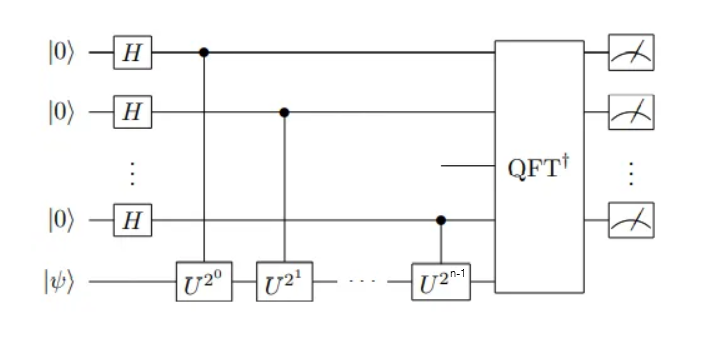
\includegraphics[scale = 0.8]{qpe_n_qubit.PNG}
  \centering
  \end{figure}

Wird die Quanten-Fourier-Transformation wie in Abbildung~\ref{fig:qpe_n_qubit} realisiert,
kann man den Zustand der Kontrollqubits vor der inversen Quanten-Fourier-Transformation wie folgt beschreiben:
\[\frac{1}{\sqrt{N}}\Bigg[
  CU^{2^0}\Big(\ket{0} + \ket{1}\Big) \tensor
  CU^{2^1}\Big(\ket{0} + \ket{1}\Big) \tensor 
  ... \tensor
  CU^{2^{n-1}}\Big(\ket{0} + \ket{1}\Big) 
  \Bigg]\]
Mit \(U^{2^x}\ket{x}_n=e^{2\pi i 2^x\varphi}\ket{x}_n\) wird der Eigenwert \(e^{2\pi i \varphi}\) wegen des Phase-Kickbacks
über die \(CU\)-Gatter auf die Kontrollqubits übertragen:
\[\frac{1}{\sqrt{N}}\Bigg[
  \Big(\ket{0} + e^{2\pi i 2^0 \varphi}\ket{1}\Big) \tensor
  \Big(\ket{0} + e^{2\pi i 2^1 \varphi}\ket{1}\Big) \tensor 
  ... \tensor
  \Big(\ket{0} + e^{2\pi i 2^{n-1} \varphi}\ket{1}\Big) 
  \Bigg]\]
Schreibt man \(\varphi\) als Binärbruch:
\[\varphi = \frac{\varphi_n}{2^1} + \frac{\varphi_{n-1}}{2^2} + ... + \frac{\varphi_1}{2^n}\]
Kann die Formel in einer ähnlichen Form wie die Quanten-Fourier-Transformation umgeformt werden:
\begin{align*}
\frac{1}{\sqrt{N}}\Bigg[
  \Big(\ket{0} + e^{2\pi i (\frac{\varphi_n}{2})} 
  ...  
  e^{2\pi i (\frac{\varphi_2}{2^{n-1}})}e^{2\pi i (\frac{\varphi_1}{2^{n}})}\ket{1}\Big) 
  \tensor ... 
  &\tensor
  \Big(\ket{0} +  e^{2\pi i (\frac{\varphi_2}{2})}e^{2\pi i (\frac{\varphi_1}{4})}\ket{1}\Big)\\ 
  &\tensor 
  \Big(\ket{0} + e^{2\pi i (\frac{\varphi_1}{2})}\ket{1}\Big) 
  \Bigg]
\end{align*}
Die Formel besitzt die gespiegelte Struktur wie die Quanten-Fourier-Transformation ohne Swap-Gatter:
\begin{align*}
  QFT_{N}\ket{x}_{n} = 
  \frac{1}{\sqrt{N}}
  \Bigg[
    \Big(\ket{0} + { e^{2 \pi i (\frac{x_1}{2})}}\ket{1}\Big) 
    &\tensor
    \Big( \ket{0} + { e^{2 \pi i (\frac{x_2}{2})(\frac{x_1}{4})}}\ket{1}\Big)\\
    &\vdotswithin{\tensor}\\
    &\tensor
    \Big(\ket{0} + e^{2\pi i (\frac{x_n}{2})} ... e^{2\pi i (\frac{x_2}{2^{n-1}})}e^{2\pi i (\frac{x_1}{2^{n}})}\ket{1}\Big)
  \Bigg]
\end{align*}
Durch die Verwendung der Swap-Gatter kann die Reihenfolge der Quanten-Fourier-Transformation gespiegelt werden, 
anschließend sind beide Formeln strukturell identisch.

Wie im Kapitel zur Quanten-Fourier-Transformation erklärt,
transformiert die Quanten-Fourier-Transformation den Zustand der Eingangsqubits \(\ket{x}_n\) in die Phasen der Ausgangsqubits.
Im Gegensatz dazu kehrt die inverse Quanten-Fourier-Transformation diesen Vorgang um, 
indem die Phaseninformationen der Eingangsqubits in Zustände der Standardbasis transformiert werden.

Die Anwendung der inversen Quanten-Fourier-Transformation, inklusive Swap-Gatter, bewirkt also:
\begin{align*}
iQFT\Bigg(
\frac{1}{\sqrt{N}}
\Bigg[
  \Big(\ket{0} + e^{2\pi i (\frac{\varphi_n}{2})} ...& e^{2\pi i (\frac{\varphi_2}{2^{n-1}})}e^{2\pi i (\frac{\varphi_1}{2^{n}})}\ket{1}\Big) \\
  &\vdotswithin{\tensor}\\
  &\tensor
  \Big(\ket{0} +  e^{2\pi i (\frac{\varphi_2}{2})}e^{2\pi i (\frac{\varphi_1}{4})}\ket{1}\Big) \tensor 
  \Big(\ket{0} + e^{2\pi i (\frac{\varphi_1}{2})}\ket{1}\Big) 
  	\Bigg]
\Bigg)
\end{align*}
\[ = \ket{\varphi_1 \varphi_{2}...\varphi_n}_n = \ket{2^n\varphi}_n\]
Schließlich kann \(\varphi\) mit einer division durch \(2^n\) bestimmt werden.

Als Beispiel wird die Quanten-Phase-Estimation für
\(U^{1\times 1}\ket{1}_1=e^{2\pi i \frac{3}{8}}\ket{1}_1\), 
also mit \(\varphi = \frac{3}{8}\) betrachtet.
Im Quantenschaltkreis aus Abbildung~\ref{fig:3_qubit_qpe} 
werden die kontrollierten \(U^{2^x}\)-Gatter als Phase-Gatter mit steigendem \(x\) in \(P(2^x 2\pi \frac{3}{8})\) realisiert.
\begin{figure} [H]
  \caption{3-Kontroll-Qubit QPE}
  \label{fig:3_qubit_qpe}
  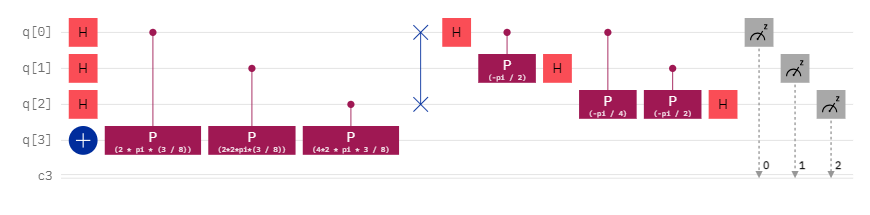
\includegraphics[width=\columnwidth]{3_qubit_qpe.png}
  \centering
  \end{figure}
Die Messung in Abbildung~\ref{fig:3_qubit_qpe_measurement} ergibt konsistent bei allen Durchläufen den Zustand \(\ket{3}_3\).
Da \(\ket{3}_3 = \ket{2^3\varphi}_3\) entspricht, 
lässt sich durch eine Division \(\varphi = \frac{3}{8}\) ermitteln.
Es ist zu beachten, 
dass die Reihenfolge der Wertigkeit der Qubits gleich bleibt.
Normalerweise tauschen die inverse wie auch die normale Quanten-Fourier-Transformation die Wertigkeiten.
Dieser Effekt wird jedoch durch Swap-Gatter korrigiert.
\begin{figure}[H]
\caption{3-C-Qubit QPE Messergebnis}
\label{fig:3_qubit_qpe_measurement}
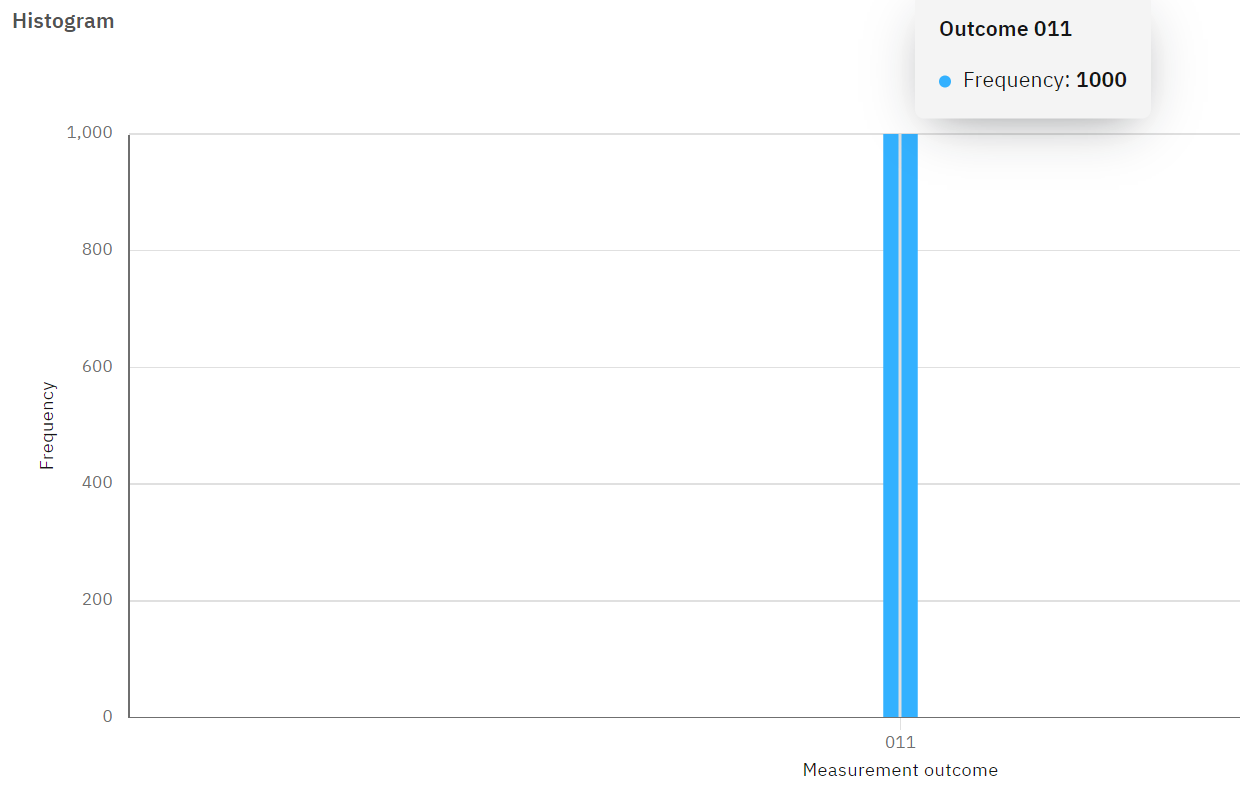
\includegraphics[width=\columnwidth]{3_qubit_qpe_measurement.PNG}
\centering
\end{figure}

Im vorherigen Beispiel liefern die Messungen aller Durchläufe den gleichen Zustand, 
durch den \(\varphi\) eindeutig bestimmbar ist.
Diese Eindeutigkeit tritt auf, 
wenn die verwendete Anzahl an Kontroll-Qubits ausreicht, 
um \(\varphi\) eindeutig zu repräsentieren.
Im obigen Beispiel kann \(\varphi\) eindeutig mit den drei verwendeten Kontrollqubits dargestellt werden:
\[{\frac{3}{8} =0 \cdot 2^{-1} + 1\cdot2^{-2} + 1\cdot2^{-3}}\]
Verwendet man nicht ausreichend Kontroll-Qubits, 
kann \(\varphi\) nicht eindeutig repräsentiert werden.
Als Konsequenz wird die Messung ungenau.
Mit hoher Wahrscheinlichkeit kollabieren die Qubits bei einer Messung 
in die darstellbaren Zustände, 
die den genauen Wert am besten approximieren.
Dabei liegt die Wahrscheinlichkeit, dass die Messung in einen der beiden angrenzenden Zustände kollabiert, 
bei \(\frac{8}{\pi^2}\)~\cite[119]{kaye2007introduction}.

In Abbildung~\ref*{fig:3_qubit_qpe_measurment_uncertain} sind die Messergebnisse einer Quanten-Phase-Estimation abgebildet, 
die die Phase \(\varphi = \frac{5}{16}\) bestimmen soll.
Da \(\frac{5}{16}\) nicht mit 3 Qubits darstellbar ist, 
gibt es kein eindeutiges Messergebnis.
Anhand der Messergebnisse ist aber erkennbar, 
dass die Messungen mit einer Wahrscheinlichkeit größer als \(\frac{8}{\pi^2}\) in
einen der beiden angrenzenden Zustände kollabiert.
Diese entsprechen \({\frac{2}{8} = \frac{4}{16}}\) und \({\frac{3}{8} = \frac{6}{16}}\), 
also genau den Werten, die \(\frac{5}{16}\) am nächsten sind.

\begin{figure} [H]
  \caption{QPE unpräzises Messergebnis}
  \label{fig:3_qubit_qpe_measurment_uncertain}
  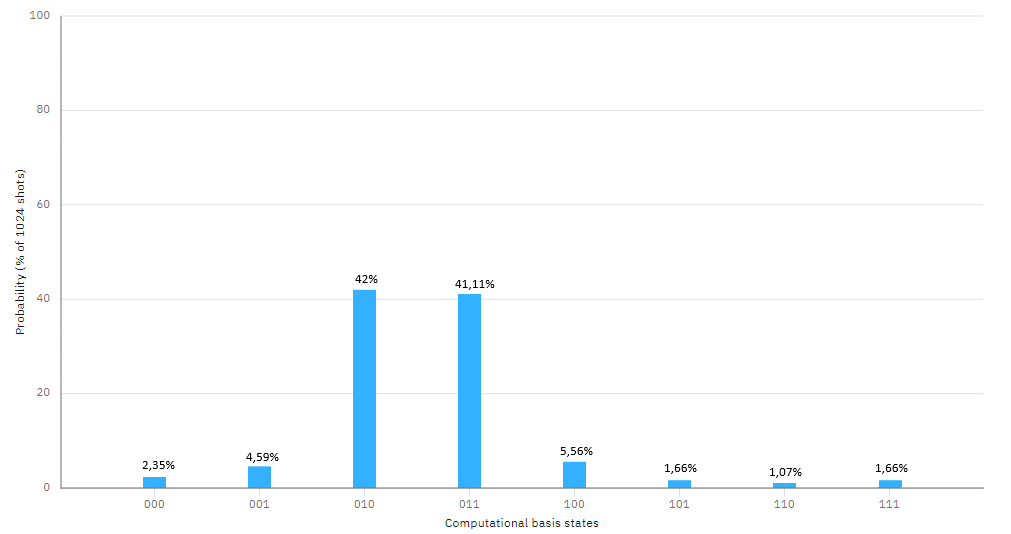
\includegraphics[width=\columnwidth]{3_qubit_qpe_measurment_uncertain.PNG}
  \centering
  \end{figure}












 






 











